\documentclass[12pt,UTF8]{ctexbook}
\usepackage{ctex}
\usepackage{array}
\usepackage{graphicx}
\usepackage{wrapfig}
\usepackage[table,dvipsnames]{xcolor}
\usepackage{tabularx}
\usepackage{longtable}
% \let\tablecaption\caption
% \let\caption\relax
\usepackage{amsmath}
\usepackage{amssymb}
\usepackage{xfrac}
\usepackage{eucal}
\usepackage{titlesec}
\usepackage{amsthm}
\usepackage{tikz-cd}
\usepackage{enumitem}
\usepackage{verbatim}
\usepackage{fontspec,xunicode,xltxtra}
\usepackage{xeCJK} 
\usepackage{caption}
\usepackage{thmtools, thm-restate}
\usepackage{tcolorbox}
\tcbuselibrary{breakable}
\tcbuselibrary{most}
% 修改脚注的编号为加圈样式,并且各页单独编号
\usepackage{pifont}
\usepackage[perpage,symbol*]{footmisc}
\DefineFNsymbols{circled}{{\ding{192}}{\ding{193}}{\ding{194}}
{\ding{195}}{\ding{196}}{\ding{197}}{\ding{198}}{\ding{199}}{\ding{200}}{\ding{201}}}
\setfnsymbol{circled}

\definecolor{gl}{RGB}{246, 252, 240}
\definecolor{gd}{RGB}{236, 244, 230}
\definecolor{bg}{RGB}{242, 244, 228}

\setCJKmainfont[BoldFont=STZhongsong, AutoFakeSlant=0.2]{STSong}
\setCJKmonofont{simkai.ttf} % for \texttt
\setCJKsansfont{simfang.ttf} % for \textsf
\setlength\parskip{8pt}
\setlength{\fboxsep}{12pt}
\renewcommand\thesection{\arabic{chapter}.\arabic{section}}
\newcommand{\arccot}{\operatorname{arccot}}
\newcommand{\dlim}[1]{^{\color{gray}\prime}#1}
\newcommand{\lian}[1]{
    \underset{#1}{\operatorname{lian}\,}
}
\newcommand{\di}[1]{\,\mathrm{d}#1}
% developpements limites
\newcommand{\oveq}[1]{\overset{#1}{=}} 
\newcommand{\olim}[1]{\mathit{o}\left(#1\right)}  % petit o
\newcommand{\Olim}[1]{\mathcal{O}\left(#1\right)}  % grand O
\newcommand{\Tlim}[1]{\mathcal{\Theta}\left(#1\right)}  % grand theta
\newcommand{\eqlim}[1]{\overset{#1}{\sim}}  % equivalence
\newcommand{\vect}[1]{\left\langle #1 \right\rangle}


\renewenvironment{proof}{\paragraph{\textbf{证明:}}}{\hfill$\square$}

\newtheorem{df}{定义}[section] 
\newtheorem{pp}{命题}[section]
\newtheorem{tm}{定理}[section]
\newtheorem{ex}{例子}[section]
\newtheorem{et}{例题}[section]
\newtheorem{sk}{思考}[section]
\newtheorem*{po}{公理}
\newtheorem*{so}{解答}
\newtheorem{xt}{习题}[section]
\newtheorem{cor}{推论}[pp]

\newtcolorbox{blk}[2][]
  {colback = white, colframe = magenta!75!black, fonttitle = \bfseries,
    colbacktitle = magenta!85!black, enhanced,
    attach boxed title to top left={xshift=5mm, yshift=-2mm},breakable, 
    title=#2, #1}

% 列举环境的行间距
\setenumerate[1]{itemsep=0pt,partopsep=0pt,parsep=0pt,topsep=0pt}
\setitemize[1]{itemsep=0pt,partopsep=0pt,parsep=0pt,topsep=0pt}
\setdescription{itemsep=0pt,partopsep=0pt,parsep=0pt,topsep=0pt}
% 章节字体大小
\titleformat{\section}{\zihao{-2}\bfseries}{ \thesection }{16pt}{}
% 封面
\title{\zihao{0} \bfseries 第四册}
\author{\zihao{2} \texttt{大青花鱼}}
% \date{\bfseries\today}
\date{}
% 正文
\begin{document}
\maketitle
\tableofcontents
\newpage

\chapter{函数的级数}

研究可微函数时,我们讨论过分析函数在某点附近的行为的问题。
我们的研究方法是:把函数在该点附近表示成多项式的形式。换句话说,我们把函数表示成一系列简单函数的和。
比如,指数函数在$0$附近可以写成:
$$e^x = 1 + x + \frac{x^2}{2} + \frac{x^3}{6} + \cdots + \frac{x^n}{n!} + \olim{x^n}.$$
那么,我们能不能把$e^x$直接写成无穷多个简单函数的和呢?

为此,我们引入了级数的概念,并证明了级数$\sum_{n\in\mathbb{N}}\frac{x^{n}}{n!}$绝对收敛。
那么,这个收敛的极限是否等于$e^x$呢?进一步来说,我们能否用多项式函数$\sum_{n=0}^N\frac{x^{n}}{n!}$
近似表示$e^x$呢?

\begin{blk}{加法结合律}
    \[(a+b)+c=a+(b+c)=a+b+c \]
\end{blk}

进一步研究仍然要用到级数。
级数除了可以用来研究数列的收敛性质,也可以用来研究函数的收敛性质。这也是级数方法更常见的应用。
不过,在此之前,我们需要做一些准备工作,比如定义什么是函数的数列,什么叫函数的收敛,等等。

\section{函数列}

给定区间$I$,我们把在$I$上有定义的实函数的集合记为$\mathcal{A}_I(\mathbb{R})$,
把其中连续函数的集合记为$\mathcal{L}_I(\mathbb{R})$,
其中$k$次可微的函数的集合记为$\mathcal{W}_I^k(\mathbb{R})$。

定义函数列为可数个函数按顺序的排列。也就是说,函数列和数列基本一样,只不过数列的每一项是函数。
比如一个由$[0,1]$上的连续实函数组成的数列:
$$ (x^2, x, 3x, 5x, \cdots (2n+1)x, \cdots )$$
它属于集合$\mathcal{L}_{[0,1]}(\mathbb{R})^{\mathbb{N}}$。

接下来定义函数列的收敛。怎么判断一个函数是否接近另一个函数呢?
与数列不同,函数列的收敛有多种定义。这里只介绍两种常用的定义。
\begin{df}{\textbf{函数列逐点收敛}}
    设有定义在区间$I$上的函数列\footnote{即“由定义在区间$I$上的函数构成的函数列”,为了方便,做一定省略。下同。}$\{f_n\}$。
    如果有定义在$I$上的函数$f$,使得对任意$r>0$,任意$x\in I$,都有正整数$N_x$,使得只要$n>N_x$,
    就有:
    $$ |f_n(x) - f(x) | < r.$$
    就说函数列$\{f_n\}$\textbf{逐点收敛}到函数$f$,$f$是$\{f_n\}$的\textbf{逐点极限}。
\end{df}

\begin{df}{\textbf{函数列一致收敛}}
    设有定义在区间$I$上的函数列\footnote{即“由定义在区间$I$上的函数构成的函数列”,为了方便,做一定省略。下同。}$\{f_n\}$。
    如果有定义在$I$上的函数$f$,使得对任意$r>0$,都有正整数$N$,使得只要$n>N$,
    就有:
    $$ \forall x\in I, \,\,\,|f_n(x) - f(x) | < r.$$
    就说函数列$\{f_n\}$\textbf{一致收敛}到函数$f$,$f$是$\{f_n\}$的\textbf{一致极限}。
\end{df}

逐点收敛是最“简单”的定义,即一个一个点来看是否越来越近。一致收敛则是从整体出发,要求所有地方的值“同时”接近,步调一致。
对比两种收敛方式,可以猜测:一致收敛的要求更高。逐点收敛时,对不同的$x$,可以有不同的$N_x$,
而一致收敛要求步调一致。

\begin{ex}
    考虑定义在$[0,1)$上的函数列$\{f_n\}_{n\in\mathbb{N}}$,其通项为:
    $$ f_n: x \mapsto \frac{nx}{e^{nx}}. $$
    对$[0,1)$中任意$x$,由于$0\leqslant x<1$,而$t$趋于无穷大时,$e^t$是$t$的高阶无穷大,因此,随着$n$增大,$nx$趋于正无穷,从而$\frac{nx}{e^{nx}}$趋于$0$。
    因此,$\{f_n\}_{n\in\mathbb{N}}$逐点收敛到$[0,1)$上的零函数。

    不过,对任意正整数$n$,取$x_n = \frac{1}{n}$,则
    $$f_n(x_n) = \frac{1}{e}.$$
    因此,只要$0<r <\frac{1}{e}$,无论$n$有多大,总有$f_n(x) = \frac{1}{e} > r$。这说明函数列$\{f_n\}_{n\in\mathbb{N}}$
    并不一致收敛到零函数。
    
    直观来看,$f_n$的图像在靠近$0$时就会隆起,即便$n$越大时,隆起的部分越来越狭窄,但高度不变。
    因此,就一致收敛的要求来说,$f_n$永远无法从整体上靠近零函数。

\end{ex}

不过,容易证明:\textbf{一致收敛的函数列,必然也逐点收敛}。

那么,一致收敛相比逐点收敛有什么优点呢?来看下面的例子。

\begin{ex}
    考虑定义在$[-1,1]$上的函数列$\{f_n\}_{n\in\mathbb{N}}$,其通项为:
    $$ f_n: x \mapsto x^{\frac{1}{2n+1}}. $$
    对$0<x<1$,$x^{\frac{1}{2n+1}}$随着$n$增大趋于$1$。
    对$-1<x<0$,$x^{\frac{1}{2n+1}}$随着$n$增大趋于$-1$。
    因此,$\{f_n\}_{n\in\mathbb{N}}$逐点收敛的极限是以下函数:
    $$
    f x\mapsto \left\{
        \begin{array}{ll}
            1 & \mbox{如果} x \in (0, 1] \\
            0 & \mbox{如果} x = 0 \\
            -1 & \mbox{如果} x \in [-1, 0) \\
        \end{array}
    \right.
    $$
    $f$在$0$处不连续。
\end{ex}
上面的例子中,
函数列$\{f_n\}_{n\in\mathbb{N}}$中每一项都是连续乃至无穷可微的函数,但它们的极限是不连续的函数。

实际应用中,我们希望把复杂的函数用简单的函数近似,在简单的函数上证明我们想要的结果,然后通过函数列收敛,
把想要的结果性质传递到原本的复杂的函数上去。
但是,如果逐点收敛不能保持极限的连续性或可微性的话,那么很多性质也无法传递到极限$f$上去。

如果函数列一致收敛的话,我们可以证明(见附录):
\begin{tm}\textbf{一致收敛保证极限}\\
    已知区间$I$上的函数列$\{f_n\}_{n\in\mathbb{N}}$一致收敛到$f$,
    且函数列的每一项$f_n$都在区间的一端$a$点处\footnote{也可以是无穷远处。}有极限$u_n$。
    那么数列$\{u_n\}$收敛到某个数$u$,且$u$是$f$在$a$处的极限。
    也就是说,在一定条件下,我们可以交换两种极限操作:
    $$ \lian{n\to +\infty} \lian{x\to a} f_n(x) = \lian{x\to a} \lian{n\to +\infty} f_n(x). $$
\end{tm}

因此,连续函数的函数列如果一致收敛,极限也是连续函数。更进一步(证明见附录):

\begin{tm}{\textbf{微变的一致极限}}
    已知函数列$\{f_n\}_{n\in\mathbb{N}}$中每一项都在区间$I$上可微,且微变函数连续。
    设函数列逐点收敛到函数$f$,且函数列$\{\partial f_n\}_{n\in\mathbb{N}}$一致收敛到函数$g$,
    那么$\{f_n\}_{n\in\mathbb{N}}$一致收敛到$f$,
    $f$在$I$上可微,且其微变函数$\partial f = g$。
\end{tm}

也就是说,在函数列收敛,且其微变函数一致收敛时,我们可以交换微变操作和函数列的极限操作:
$$ \lian{n\to +\infty} \partial f_n = \partial \lian{n\to +\infty} f_n. $$

\section{幂级数}

\section{收敛半径}

\chapter{连续函数的和}

小学的学习中,我们定义了有限个数的和。通过定义级数,我们学习了无穷多个数的求和。
不过,正如我们所知,无穷也有可数与不可数之分。级数定义了可数多个数的求和。
那么,是否能对不可数多个数求和呢?

举例来说,实数集是不可数集合,实数区间中的点也是不可数集合。
给定定义在实数集或某个区间$I$上的实变函数$f$,它将集合中每个点映射到函数值$f(x)$。
那么,能否对这些函数值求和呢?

这个问题比可数多个数的求和更为复杂,但在实际生活与生产中经常出现。
比如,我们通常假设时间是连续变量,而评估各种物理作用的效果时,通常需要研究一段时间内作用的效果。
例如,物体受的力在一定时间内的累计效果,称为冲量。它是物体导致速度变化的因素。
设物体在$t$时刻受力为$F(t)$,那么,
一段时间$[t_1, t_2]$上的冲量就是函数$F(t)$在$[t_1, t_2]$的累积。

另一个例子是带电物体的电荷累计。我们假设物体表面每个点上的电荷是连续分布的,一点$P$上的电荷密度是$g(P)$。
那么,物体表面的总电荷就是表面所有点上电荷密度的累积。

因此,我们有必要定义函数在区间、平面区域乃至更复杂的形体上的求和。
良好的定义并不是显而易见的。为这类求和给出符合实际生产生活中的需要的定义,
是一门深奥的学问。在当前阶段,我们只给出简要的介绍,研究特定情形下的求和工具,不作更深入的探索。

\section{函数图像的面积}

首先来看一个物理学中的例子。设物体受到方向恒定,大小随时间$t$变化的力$F(t)$。
定义$F(t)$在一段时间内的累积效果为冲量$I$。如果设物体刚受力时的冲量$I(0) = 0$,那么有定律:
$$ I(t) - I(0) = m(v(t) - v(0)).$$
其中$v$是物体的在受力方向上的速率。为了计算速率的改变量,我们希望计算$I(t)$,也就是$F(t)$的“和”。

以时间为横轴,画出函数$F$的图像。如果$F$的大小也是恒定的,
那么可以发现,$F$在一段时间$[t_1, t_2]$内的“总和”就是$F \cdot (t_2 - t_1)$。
从图像来看,函数图像是水平的线段,$F(t)$的“和”就是函数图像与$x$轴之间的矩形的面积。

如果物体受力大小不恒定,但分段恒定,于是函数图像可以看作若干段水平线段。
于是,按分段求多个矩形的面积,然后求和,就得到$I$的改变量。

然而,更常见的情况是:$F$的大小随时间不断改变。这时候,我们如何求$F$的“和”呢?

需要知道的是,对一般的函数$F$,我们并不能很好地定义$I$的改变量。不过,对于物理学中常见的模型
以及当前我们接触的简单形状来说,可以用比较简单的方法,定义“函数曲线的面积”。

具体来说,$F$恒定或分段恒定的情形下,我们计算矩形的面积。从这个方法出发,对一般的函数$F$,
我们也希望用一系列的矩形来近似表示“函数曲线的面积”。

% \begin{figure}[h] %this figure will be at the right
%     \vspace{4pt}
%     \centering
%     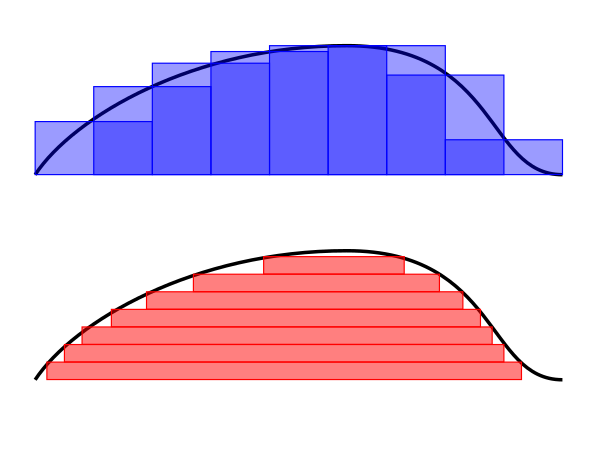
\includegraphics[width=0.4\textwidth]{tu/积分定义5.png}
%     \caption*{\texttt{用矩形近似表示函数曲线下方的面积}}
% \end{figure}

% 具体的方法有两种。一种是把区间$[t_1, t_2]$竖直分割成很多段,把每段的函数曲线近似看作水平线段,
% 这样就得到一系列左右并排的、“竖直”的矩形。另一种是把函数曲线下方的区域横着分割,得到一系列上下相叠、高度相同,
% 但长度不同(由函数性质决定)的矩形。

% 无论用哪种方法,如果只要矩形足够“细”,矩形面积就趋于某个极限,那么我们就把这个极限看作$F$的“和”。

% 那么,怎样严格地说明这个定义呢?两种方法中,第一种方法可以用我们已经学过的概念严格说明。
% 因此,我们目前采用第一种方法来定义。

\begin{df}{\textbf{区间的分割}}
    \mbox{} \\
    给定闭区间$I=[a, b]$及一列从小到大排列的数$a = x_0 < x_1 < \cdots < x_{n-1} < x_n = b$。
    则把区间$I$分成$n$个子区间$[x_0, x_1], \,\,\, [x_1, x_2], \,\,\,\cdots, \,\,\,[x_{n-1}, x_n]$,就是这一列数对区间的分割。
    我们用数列$(x_0, x_1, \cdots, x_n)$表示这个分割。

    如果区间的分割有$n$个子区间,就说它是区间的$\boldsymbol{n}$\textbf{阶分割}。
    如果区间的分割使得所有子区间长度都不超过某个数$d$,就说它是区间的$\boldsymbol{d}$\textbf{–分割}。

    % 设$f$是定义在$I$上的函数。给定区间的某个分割,
    % 在该分割的各个子区间中取样$c_i\in [x_{i-1}, x_{i}]$,其函数值$f(c_i)$与区间长度的乘积的总和:
    % $$ \sum_{i=1}^n (x_i - x_{i-1}) f(c_i) $$
    % 称为函数关于该分割的\textbf{取样和}。
\end{df}

给定区间$I$上的函数$f$和区间$I$的分割,如果$f$在分割的每个子区间上都是常函数,就说$f$是\textbf{分段常函数},也叫\textbf{阶梯函数}。

举例来说,

\begin{figure}[h] %this figure will be at the right
    \vspace{4pt}
    \centering
    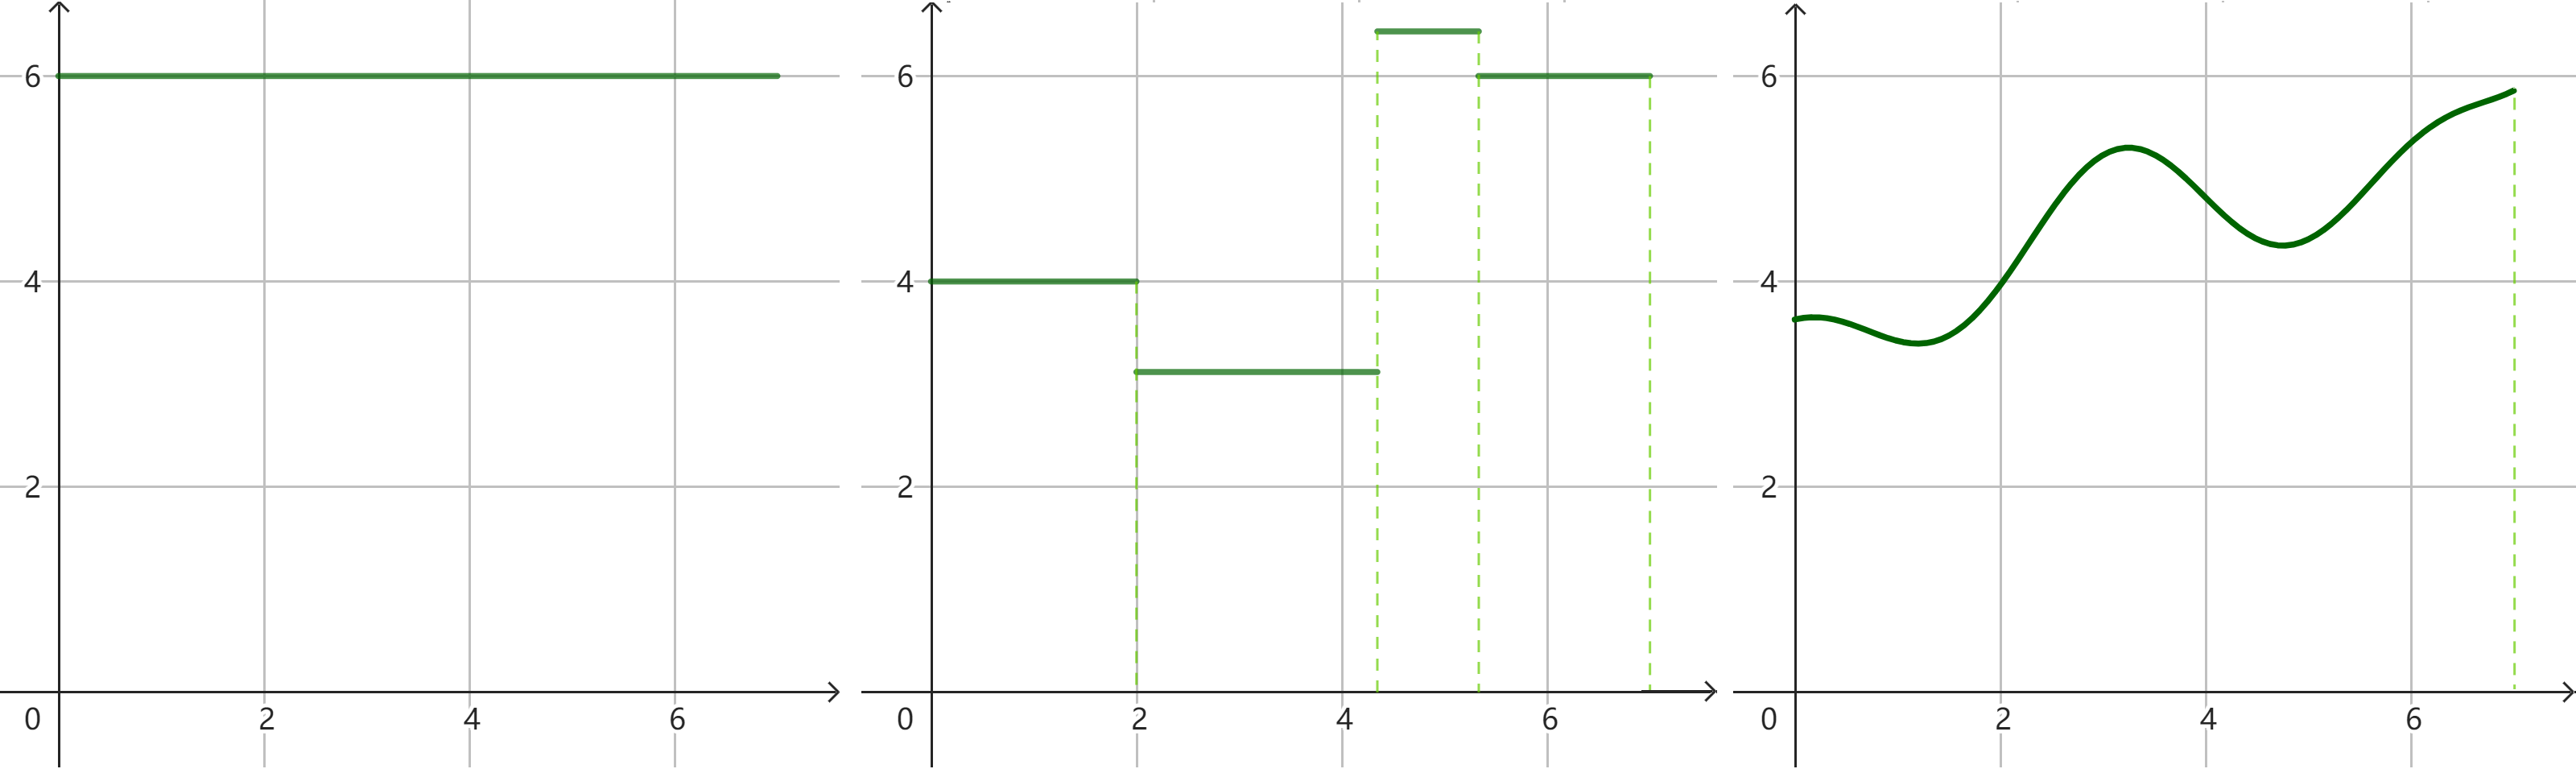
\includegraphics[width=0.8\textwidth]{tu/积分定义1.png} %  KSmrq,CC BY-SA 3.0,https://commons.wikimedia.org/w/index.php?curid=2335935
    \caption*{\texttt{左一、左二是阶梯函数,右一不是阶梯函数}}
\end{figure}

\begin{df}{\textbf{阶梯函数的积合}}
    设有定义在闭区间$I=[a, b]$上的阶梯函数$f$,对应分割$(x_0, x_1, \cdots , x_n)$。
    设$f$在子区间$[x_i, x_{i+1}]$的函数值为$c_i$,则$f$在区间$I$上的\textbf{积合}定义为:
    $$ \sum_{i=0}^{n-1} c_i(x_{i+1} - x_i).$$
    
    $f$在区间$I$的积合记为
    $$ \int_I f(x)\di{x} \quad \mbox{或} \quad \int_a^b f(x)\di{x} $$
\end{df}

直观上看,把阶梯函数到$x$轴之间的部分看作一系列左右并排的矩形,阶梯函数的积合就是矩形面积的和。

对一般的函数来说,是否能定义积合呢?我们采用逼近的思想。给定区间$I$上的函数$f$,
我们可以找与$f$的曲线类似的阶梯函数。用这样的阶梯函数的积合,来近似定义$f$的函数曲线的面积。
如果随着阶梯函数与$f$“越来越像”,它的积合趋于一个固定的极限值,那么,我们可以定义这个极限为$f$的函数曲线的面积。




% \begin{figure}[h] %this figure will be at the right
%     \vspace{4pt}
%     \centering
%     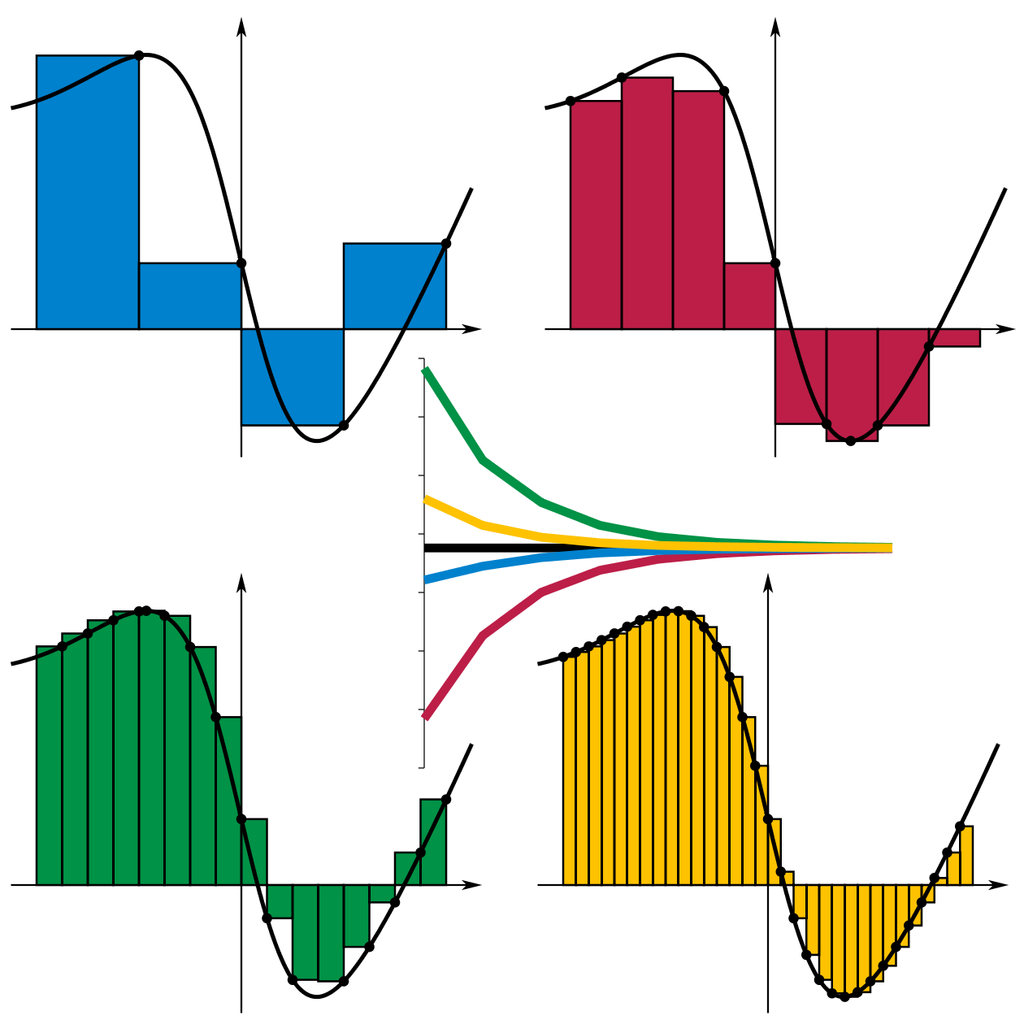
\includegraphics[width=0.5\textwidth]{tu/积分定义6.png} % from KSmrq,CC BY-SA 3.0,https://commons.wikimedia.org/w/index.php?curid=2347919
%     \caption*{\texttt{不同的取样方法,随着分割越来越细,取样和面积收敛}}
% \end{figure}

% 从定义中可以看出,我们并不保证函数在任何闭区间上都能定义积合。
% 如果函数在某个区间上无法定义积合,就说它在该区间上不可积。
% 不过,我们接下来会看到,很多我们接触过的常见显式函数,都是可积的。

% 定义中,我们假设函数总在$x$轴上方。如果函数有小于$0$的值,如何定义积分呢?

% 设函数在$[a,b]$上求积。首先,如果函数$f$总小于零,它的图像总在$x$轴下方。它与$x$轴之间的面积可以说是“函数曲线上方的面积”。
% 我们可以定义它的积合是$-f$积合的相反数。

% 如果函数值有正有负,$x$轴把函数曲线分为上下两个部分。我们可以把$x$轴上方部分和$x$轴之间的面积记为正,
% 把$x$轴下方部分和$x$之间的面积记为负。函数在区间上的积合就是正负面积之和。

% 另一种定义方法是先把坐标轴往下平移,即用$y = -a $代替$x$轴。
% 其中$a$是足够大的数,使得函数在区间上的值总大于$-a$。这样,我们定义

% 具体来说,给定函数,如何求它在区间上的积合呢?

% 从最简单的函数$f: x\mapsto x$出发。我们想知道它在区间$I = [0, 1]$上的合。

% 把区间$I$做$n$–分割后取样,取样和为:
% $$ S_n = \sum_{i=1}^n (x_i - x_{i-1}) f(c_i) = \sum_{i=1}^n (x_i - x_{i-1}) c_i. $$
% 其中$0 = x_0 < x_1 < \cdots < x_n = 1$,$x_{i-1} \leqslant c_i \leqslant x_i$。

% 于是,
% $$ x_{i-1}^2 - x_i x_{i-1} = (x_i - x_{i-1}) x_{i-1} \leqslant (x_i - x_{i-1}) c_i \leqslant (x_i - x_{i-1}) x_i = x_i^2 - x_{i-1} x_i $$
% 而
% $$ \sum_{i=1}^n x_i^2 - x_{i-1} x_i = \sum_{i=1}^n \frac{x_i^2 - x_{i-1}^2}{2} + \frac{(x_i - x_{i-1})^2}{2} = \frac{x_n^2 - x_0^2}{2} + \sum_{i=1}^n\frac{(x_i - x_{i-1})^2}{2}. $$
% $$ \sum_{i=1}^n x_{i-1}^2 - x_i x_{i-1} = \sum_{i=1}^n \frac{x_i^2 - x_{i-1}^2}{2} - \frac{(x_i - x_{i-1})^2}{2} = \frac{x_n^2 - x_0^2}{2} - \sum_{i=1}^n\frac{(x_i - x_{i-1})^2}{2}. $$
% 所以,
% $$ \left| S_n - \frac{x_n^2 - x_0^2}{2} \right| \leqslant \sum_{i=1}^n\frac{(x_i - x_{i-1})^2}{2} $$
% 注意到$x_0$、$x_n$是定值,而对于$d$分割来说,$x_i - x_{i-1}$总小于$d$。取$d = \frac{1}{n}$,就有
% $$ \left| S_n - \frac{x_n^2 - x_0^2}{2} \right| \leqslant \frac{1}{n}. $$
% 因此,随着分割越来越细,$S_n$趋于$\frac{x_n^2 - x_0^2}{2} = \frac{1}{2}$。$f$在$I$上的合是$\frac{1}{2}$。

% 对于一般区间$[a, b]$,同理可得$f$在$[a, b]$上的合是$\frac{b^2 - a^2}{2}$。

% 可以看到,即便对最简单的函数,求合也不是显而易见的事情。我们在推导中也用到了一些技巧。
% 那么,一般来说,对于更复杂的函数,如何求合呢?甚至,如何确定它们可积呢?
% 且听下回分解。

\begin{sk}
    \mbox{} \\
    \indent 1. 对比函数的积合与微变,它们有哪些类似之处?有哪些不同之处?\\
    \indent 2. 函数关于区间分割的取样和,与关于函数微变哪个定理有相似之处?你有什么想法?\\
    \indent 3. 使用上下相叠的矩形来定义积合,需要注意哪些问题?\\
    \indent 4. 如果函数在区间$[a, b]$上某点无定义,是否还能定义它在区间上的积合?要注意哪些问题?
\end{sk}

\section{函数的定合}
\section{合函数}

\chapter{方程与空间}

\chapter{复数}

\begin{appendix}

\chapter{函数的级数}
\begin{tm}{\textbf{一致收敛保证极限}}
    已知区间$I$上的函数列$\{f_n\}_{n\in\mathbb{N}}$一致收敛到$f$,
    且函数列的每一项$f_n$都在区间的一端$a$点处\footnote{也可以是无穷远处。}有极限$u_n$。
    那么数列$\{u_n\}$收敛到某个数$u$,且$u$是$f$在$a$处的极限。
    $$ \lian{n\to +\infty} \lian{x\to a} f_n(x) = \lian{x\to a} \lian{n\to +\infty} f_n(x). $$
\end{tm}

\begin{tm}{\textbf{一致收敛传递连续性}}
    连续函数的函数列如果一致收敛,极限也是连续函数。
\end{tm}

更进一步有:

\begin{tm}
    如果函数$f$在区间$I$上可微,且微变函数在$I$上连续,就说$f$在$I$上\textbf{一阶光滑}或\textbf{连续可微}。
    如果$f$的前$k$次微变都在$I$上一阶光滑,就说$f$在$I$上$\boldsymbol{k}$\textbf{阶光滑}或$\boldsymbol{k}$\textbf{阶连续可微}。
    如果对任意正整数$k$,$f$在$I$上$k$阶光滑,就说$f$在$I$上\textbf{光滑}。

    已知函数列$\{f_n\}_{n\in\mathbb{N}}$中每一项都在区间$I$上可微,且微变函数连续。
    设函数列逐点收敛到函数$f$,且函数列$\{\partial f_n\}_{n\in\mathbb{N}}$一致收敛到函数$g$,
    那么$\{f_n\}_{n\in\mathbb{N}}$一致收敛到$f$,
    $f$在$I$上可微,且其微变函数$\partial f = g$。

    也就是说,在一定条件下,我们可以交换微变、极限和函数列的极限操作:
    $$ \lian{n\to +\infty} \partial f_n = \partial \lian{n\to +\infty} f_n. $$

    如果函数列$\{f_n\}_{n\in\mathbb{N}}$中每一项都在区间$I$上$k$阶连续可微,简单收敛到某个函数$f$,并且
    \begin{enumerate}
        \item 对任意$1 \leqslant i < k$,函数列$\{\partial^i f_n\}_{n\in\mathbb{N}}$简单收敛到函数$g_i$;
        \item 对任意闭区间$B \subseteq I$,函数列$\{\partial^k f_n\}_{n\in\mathbb{N}}$在$B$上一致收敛到函数$g_k$。
    \end{enumerate}
    那么$f$在$I$上$k$阶连续可微,且其前$k$阶微变函数为$\partial^i f = g_i$($1 \leqslant i\leqslant k$)。
    此外,$\{f_n\}_{n\in\mathbb{N}}$在$I$中任意闭区间一致收敛到$f$。

\end{tm}

\end{appendix}

\end{document}